\section{Model-Based RL}\label{sec:model-based}
In the previous section Actor-Critic methods were implemented on both the CartPole and Catch environments. The inclusion of an inductive bias exploiting the symmetry of an MDP lead to improvements in the sample efficiency of learning an expert policy, while maintaining robustness to initialization conditions.

In the case where the transition dynamics of the MDP are group structured, or approximately group structured, this report proposes the use of an Equivariant world model. With a world model that has inductive biases that are designed to aid in learning the MDP's transition dynamics, the world model may be learned more efficiently and accurately from fewer samples from the environment, improving the effectiveness of planning for the agent.

The specific algorithm implemented to create a model-based agent is a Dyna~\ref{sec:Dyna} algorithm, with a PPO \ref{sec:PPO} agent. Using the Dyan-PPO agent, means that when the number of planning steps is set to zero, the agent becomes a model free PPO agent, enabling direct comparison with the baseline MLP PPO implemenation~\ref{sec:baseline}.

Both, Catch and CartPole are environments where the reward function is only a function of the state the agent is in and not a state-action pair. Further, their rewards are simple functions of their state, this report forgoes learning the reward dynamics of the environments, and use their existing reward structure on simulated states such that,
\begin{equation}
	R_{t+1} = R(T(s, a)).
\end{equation}
Where, $R$, is the reward function defined by the environment.

\subsection{Constructing Transition Models}
Before using a full model-free algorithm, where the model is learned online, during the training. A simplified algorithm, Supervised-Dyna, is tested that uses off-line trained world models. The process for this is outlined below:
\begin{algorithm}
	\label{alg:Supervised-Dyna}
	\caption{Supervised-Dyna}
	\begin{algorithmic}
		\State Initialize $T_\phi$
		\State Sample transition tuples from a policy $\pi \sim (s, a, s')$ on MDP $\mathcal{M}$.
		\Comment {Here $\pi$ is a random/ expert policy}
		\State Form Dataset $\mathcal{D}$ from sampled transition tuples.
		\For {Num Epochs}
		\State $\phi' \leftarrow $Minimise $L(\phi , \mathcal{D})$.
		\EndFor
		\For {Num Dyna Iterations}
		\For {Num Acting Updates}
		\State Sample transition tuples from policy $\pi_\theta \sim (s, a, s')$ on $\mathcal{M}$
		\State Train agent $\pi_\theta$ from direct samples.
		\EndFor
		\For{Num Planning Updates}
		\State Sample transition tuples from policy $\pi_\theta \sim (s, a, s')$ on $T_\phi$.
		\State Train agent $\pi_\theta$ from planned samples.
		\EndFor
		\EndFor
	\end{algorithmic}
\end{algorithm}

Using off-line trained world models has benefits as an intermediate step. Firstly, the world model is stationary throughout the agent training process and can be easily investigated. Secondly, the model can be trained with ample data. This is in contrast to full Dyna where, the length of the planning and acting phases must be tuned as a hyperparameter, and the convergence of the models must be tuned. This hyperparameter of $\text{Num Acting Updates}/\text{Num Planning Updates}$, is referred to as the Planning ratio.


\subsection{Proximal Pooling Motivation}

To produce equivariant world models, there are additional challenges beyond that of just implementing a G-CNN which permutes its outputs dependent on the input transformation. In contrast to an equivariant actor where simply permuting the logits of a distribution suffices to have equivariant behaviour \ref{symmetrizer}. When building an equivariant world model with a G-CNN, the output of the network predicts the next state and a number of nonsense next states.

To illustrate what the final layer output in the G-CNN is doing, consider the same setup as the Actor-Critic networks, where there is a hidden representation that's responses get permuted depending on the application of a group structured transformation on the input:

\begin{equation}
	f(s , a) = \begin{pmatrix}
		g(s, a)                                     \\
		g(\ell_1^\mathcal{S}s,\ell^\mathcal{A}_1a)  \\
		g(\ell^\mathcal{S}_2s, \ell^\mathcal{A}_2a) \\
		\vdots                                      \\
		g(\ell_{|G|}^\mathcal{S}s, \ell^\mathcal{A}_{|G|}a),
	\end{pmatrix}
\end{equation}
and when a transformation is applied to the input these responses, $g$ are permuted,
\begin{equation}\label{eq:tm_gcnn}
	f(\ell_i^\mathcal{S}s, \ell_i^\mathcal{A}a) = \mat{P}_i f(s, a).
\end{equation}
Because the permutations are defined by the group, these are the same permutations as in Eq.\ref{eq:gs_perm}. However here each response $g: \mathcal{S} \times \mathcal{A} \rightarrow \mathcal{S}$. In order to get a transition function there must be a method to pool over the responses.

\subsection{Group Action Transformation}
When the network $f$ performs a forward pass and outputs the vector of responses, Eq.\ref{eq:tm_gcnn}, the equivariance in the response is mapping group actions on a state space to a permutation of responses that are all the same shape as the state. This is not the equivariance constraint that is required for a transition model, which is,
\begin{equation}
	T(\ell_i^\mathcal{S}s, \ell_i^\mathcal{A}a) = \ell_i^\mathcal{S}T(s, a).
\end{equation}
The first step in achieving this is to apply a group action to each row of the response of $f$. This is the Action Transformation operation denoted as $\mat{\mathcal{T}}$, where,
\begin{equation}
	\mat{\mathcal{T}}f(s,a) = \begin{pmatrix}
		g(s, a)                                                          \\
		\ell_{-1}^\mathcal{S}g(\ell_1^\mathcal{S}s,\ell^\mathcal{A}_1a)  \\
		\ell_{-2}^\mathcal{S}g(\ell^\mathcal{S}_2s, \ell^\mathcal{A}_2a) \\
		\vdots                                                           \\
		\ell_{-|G|}^\mathcal{S}g(\ell_{|G|}^\mathcal{S}s, \ell^\mathcal{A}_{|G|}a)
	\end{pmatrix}.
\end{equation}
Due to group closure, this gets us quite close to equivariance! For example consider some group element, which is the inverse of $i$ acting on the input,

\begin{equation}\label{eq:g-cnn}
	\mat{\mathcal{T}}f(\ell_{-i}^\mathcal{S}s,\ell_{-i}^\mathcal{A}a) = \begin{pmatrix}
		g(\ell_{-i}^\mathcal{S}s,\ell_{-i}^\mathcal{A}a)                 \\
		\ell_{-1}^\mathcal{S}g(\ell_j^\mathcal{S}s,\ell^\mathcal{A}_ja)  \\
		\ell_{-2}^\mathcal{S}g(\ell^\mathcal{S}_ks, \ell^\mathcal{A}_ka) \\
		\vdots                                                           \\
		\ell_{-i}^\mathcal{S}g(s, a)                                     \\
		\vdots                                                           \\
		\ell_{-|G|}^\mathcal{S}g(\ell_{|G|}^\mathcal{S}s, \ell^\mathcal{A}_{|G|}a)
	\end{pmatrix}.
\end{equation}
Then to achieve equivariance, the correct row must be selected. This would be straightforward if the group action on the input was known, but in general it is not. However, in many cases, in a transition model, the output is closer to the input than any of the other states! With this proximity intuition a pooling method is introduced to gain approximate equivariance with the transition models. This vector of next states, is referred to as transition images.

When using CNNs or other G-CNNs for classification or other image processing tasks, a reduction pooling such as mean or max is used over the different groups. Both of these pooling types result in an invariant network, where, if one pools over the group, takes a mean or a max over the group dimension of $f$, because the transformation only applies a permutation along this axis there is no change in the output if the group dimension is permuted,
\begin{equation}
	\max_\text{axis G} \mat{P}_i f(s, a) = \max_\text{axis G} \mat{P}_j f(s, a), \forall i, j.
\end{equation}
Here the group axis, axis G, is the leading dimension in $f$ if $f: \mathcal{S} \times \mathcal{A} \rightarrow \mathbb{R}^{|G| \times \mathcal{S}}$. This invariance is not helpful in our case and so an alternative technique of pooling over possible next states is proposed.


\subsection{Proximal Pooling Layers}\label{sec:proximal_pool}
As a forward, this method does not guarantee equivariance to the input transformation. However, empirically it is effective.
The proximal pooling layer, $\mathcal{P}$, takes a distance metric, $d(s, s')$, and selects the transition image, which has the minimum distance metric, as such the full approximately equivariant network is;
\begin{equation}
	T(s, a) = \mathcal{P}\mathcal{T}f(s, a)  =\arg \min_\text{axis G} d \left (s,  \begin{pmatrix}
			g(s, a)                                                          \\
			\ell_{-1}^\mathcal{S}g(\ell_j^\mathcal{S}s,\ell^\mathcal{A}_ja)  \\
			\ell_{-2}^\mathcal{S}g(\ell^\mathcal{S}_ks, \ell^\mathcal{A}_ka) \\
			\vdots                                                           \\
			\ell_{-|G|}^\mathcal{S}g(\ell_{|G|}^\mathcal{S}s, \ell^\mathcal{A}_{|G|}a)
		\end{pmatrix}
	\right ).
\end{equation}
The $\arg \min_\text{axis G}$, returns the state image, which is closest to the original state, if the network predictions are better than random with respect to the distance metric.

Empirically across 10,000 randomly sampled CartPole states, the network, $T(s, a)= \mathcal{P}\mathcal{T}f(s,a)$, is fully equivariant, when untrained. When trained, it is equivariant across the same sample, and also achieves better validation MSE than the non equivariant model, when trained on transitions from the same data.

This is not the case for the Catch network. Catch has $675$ state action pairs, and the transition model when untrained achieves $98.3 \pm 0.6\%$ equivariance, across all these state action pairs. The standard error is quoted over 1000 random seed parameter initializations. The performance of the transition models is investigated in more depth, in sections\ref{something,something}.

When trained, the Catch model is able to achieve validation accuracy of 1. As such, the lack of perfect equivariance, may not be an issue in some scenarios. Small discrete spaces, with a high degree of symmetry are the worst in terms of a lack of equivariant predictions, as the expected distance between any two states decreases. Additionally, for MDPs where no sensible distance metric can be constructed this method will fail.
\begin{proposition}
	Given some distance metric between two states $d(s, s')$ and a G-CNN transition model of the form Eq.\ref{eq:g-cnn}. If at some time $t$ a state transition from $s_t$ to $s_{t+1}$ takes place. And the MDP has a group structured discrete symmetry, if the state space obeys,
	\begin{equation}
		d(s_t, s_{t+1}) < \mathbb{E}_{s'\sim \mu}[d(s_t, s')], \forall i, s_t.
	\end{equation}
	Where $\mu$ is the steady state distribution. Then, a proximal pooling layer can be used to make the G-CNNs' forward pass approximately equivariant.
\end{proposition}
As motivation for why this is, when the G-CNN performs a forward pass, one of the multiple outputs of $\mathcal{T} f(\ell_i^\mathcal{S}s,\ell_i^\mathcal{A} a)$, are empirically not correlated to the other group members, for all parts of the state effected by the transformations.
\begin{figure}[h!]
	\centering
	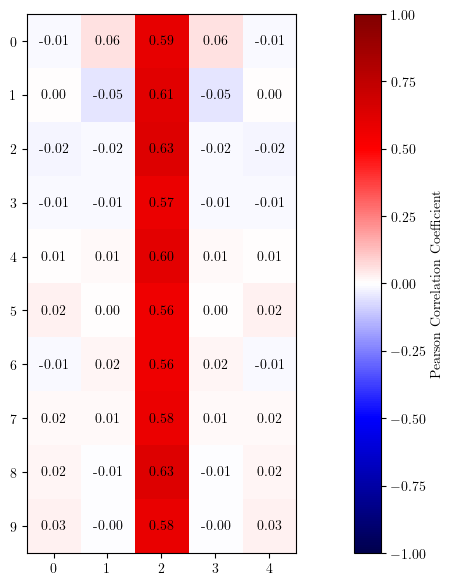
\includegraphics[width = 0.5\textwidth]{Figures/logits_correlation.png}
	\caption{Pearson $r^2$ value for each logit in the ouput of the transition model between $g(s, a)$ and $\ell_r^\mathcal{S}g(\ell_r^\mathcal{S}s,\ell_r^\mathcal{A}a)$, for one of the 675 possible sate action pairs, across 1000 random  seeds for network initialization. }
	\label{fig:logits_correlation}
\end{figure}
Empirically one can see the lack of correlation in Fig.\ref{fig:logits_correlation}, which plots the $r^2$ co-efficient between the transition images across 1000 randomly initialized untrained networks. The network parameterize the next states as two distributions, by outputting an array of 50 logits. As expected, the network responses along the centre axis should be invariant to the input transformation. Thus, a positive correlation co-efficient is encouraging. For all other logits in the distribution over the next state there is no evidence of a correlation between the two transition images, at a 5\% significance level.

With the two outputs being independent of each other, then correct next state can be selected using the proximal layer reliably, and the networks can be approximately equivariant.



\subsection{CartPole}
A CartPole transition model is a functional approximation to a deterministic Non-linear system.
To learn this transition model, transitions are sampled from a policy on the MDP, and stored. This is then used as a dataset to perform supervised learning on. The Transition model, $T_\phi: \mathcal{S} \times \mathcal{A} \rightarrow \mathcal{S}$, predicts next states from a state action pair.

The loss function for the transition model is the average L2 distance between the predicted next state, and the true next state across a batch of samples.
\begin{equation}
	L(\phi) = \frac{1}{N}\sum^N_{(s, a, s')_i \sim \mathcal \tau} ||T(s, a) - s'||_2
\end{equation}
Here $\tau = \{(s, a , s')_1^N\}$ is a batch of transition, of size $N$, sampled from the MDP, and $(s, a, s')$, is the state, action, next state tuple. Often a reward model is required to also make an MDP. For simplicity, the CartPole reward model is used, rather than learned. As such the transition gains a reward of $+1$, if $|\theta| < 12.5^o$, otherwise the episode terminates.

\subsubsection{Constructing Equivariant World Models}
Like in the previous section on \ref{sec:actor-critic}, the equivariant transition models are deep G-CNNs. In contrast to equivariant Actors in the previous section, these networks have to use the proximal pooling layer on their output \ref{sec:proximal_pool}. The equivariance described by these nextworks is to the identity and negative operation, such that;
\begin{equation}
	T(- s, 2*a - 1) =  -T(s, a), \forall
\end{equation}
These transition models, are not truely equivariant but empirically the proximal pooling layer suffices to meet the equivariance condition. As a distance metric to achieve the equivariance, the proximal pool uses the $L1$ distance.

Again in a similar fashion to the actor networks, the transition models have two hidden Group Covolution layers. The input layer for actions also transforms the action from $[0, 1]$ to $[-1, 1]$. Thus the same group convolution layer can be used for both the state and the action input.


\subsubsection{Results: Comparing Convergence of Transition Models}
In order to perform model based RL a transition model must be learnt to simulate transitions, such that the agent can learn a policy that performs better in the original environment. Thus the first set of experiments were training transition models in a supervised learning setting.

Three different pairs of models were trained. The first pair on data collected from an expert and random policy. The second pair took the first dataset and filtered out the transitions which took the right action. The final pair is trained only on data sampled from a random policy.
\begin{figure}
	\centering
	\includegraphics*[width=\linewidth]{Figures/transition_model_cp.png}
	\caption{Transition Model RMS error, plotted against epochs for three different training datasets. Left, the dataset contains a 50/50 split between expert policy sampled transitions, and transitions sampled from a random policy. Center, the same dataset as left, however, with only the left action taken. Right, solely transitions sampled from a random policy. These datasets contain 40,000 transitions. All plots have the same set of validation data with a 50/50 split of expert and radom policy sampled data.}
	\label{fig:transition_model_cp}
\end{figure}
In Fig.\ref{fig:cartpole_equivariant_actor} it is clear that the G-CNN despite having the same parameter count, performs similarly or better on all three transition datasets. Further, there is a reassuringly stark delta in performance between the equivariant model, and the conventional MLP transition model, when the right action is filtered out. The equivariant model recovers the majority of the performance in this scenario, while the MLP appears to overfit to left actions heavily. When it is asked to generalise to transitions that it has not seen it fails. Interestingly, when only random data is sampled The equivariant model has lower validation loss. To further investigate this, the final transition model validation loss is plotted by angle, for each of the datasets in Fig.\ref{fig:cp_model_angle}.

Interestingly, when looking at the left hand figure, the RMS error is substantially higher for the equivariant model, for $\theta <|5^o|$. Indicating that the equivariant constraints and the structure of the model limit the accuracy of the model in comparison to the MLP. However, the delta in mean validation loss between the two, models over all angles is very similar, with both models having a mean validation loss of $0.013$, to two significant figures over the entire dataset. As the losses are dominated by the larger angles, where the transition dynamics are much less linear due to the moments applied to the cart by the pole's acceleration.
\begin{figure}[h!]
	\label{fig:cp_model_angle}
	\begin{center}
		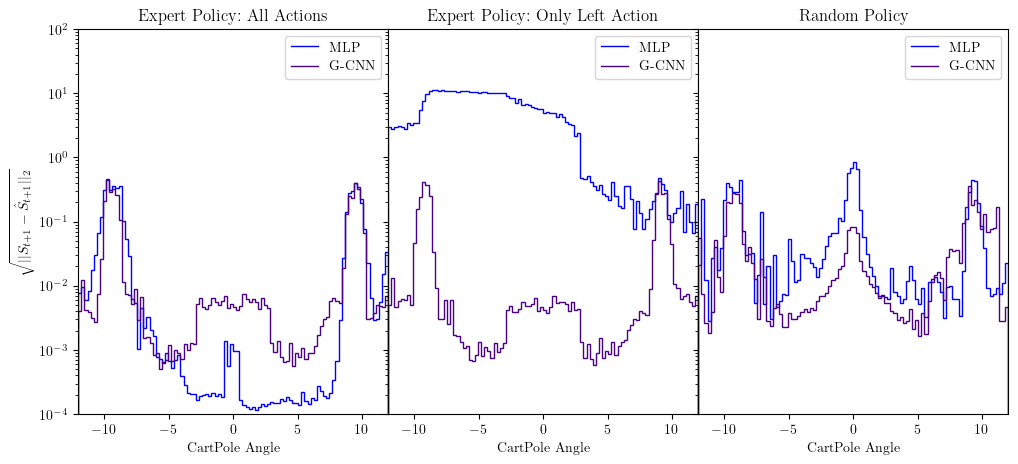
\includegraphics[width=0.95\textwidth]{./Figures/transition_model_cp_angle.png}
	\end{center}
	\caption{RMS Error plotted by angle on validation transitions sampled from a 50/50 split of expert and random data. Left, models trained on a dataset of 50/50 sampled expert and random policy transitions. Center, only transitions taking the left action. Right, transitions only sampled from a random ploicy.}
	\label{fig:}
\end{figure}

On the other two datasets, the story is slightly different. When trained on only the left action, the power of the equivariant generalisation is very impressive with the model recovering very similar RMS error, overall and when divided by angle. Demosntrating the advantage of equivariance as and inductive bias.
In the last plot, where the model is trained solely on transitions sampled from random actions, an interesting result is obtained. The equivariant model performs notably better across all angels, with an RMS validation error of $0.049$, in comparison of that to the MLP of $0.19$. On validation data that is sampled jointly from an expert policy, where the majority of transitions are at small angles. This improved generalisation, from the random dataset to a dataset that posseses more transitions in the low angle range may be important in training Dyna Agents, where initially the Agents policies are suboptimal, but they learn in the simulated environment. Thus, improved model generalisation to transitions more frequently chosen by an optimal policy may provide an uplift in Model based agent performance.\footnote{The transition distributions can be found in the Appendix.\ref{ap:dist_cp}.}

\subsubsection{Results: Supervised-Dyna}
Using the off-line trained world model above, the Actor-Critic agent was trained using the Supervised-Dyna algorithm~\ref{alg:Supervised-Dyna}.
\begin{figure}
	\centering
	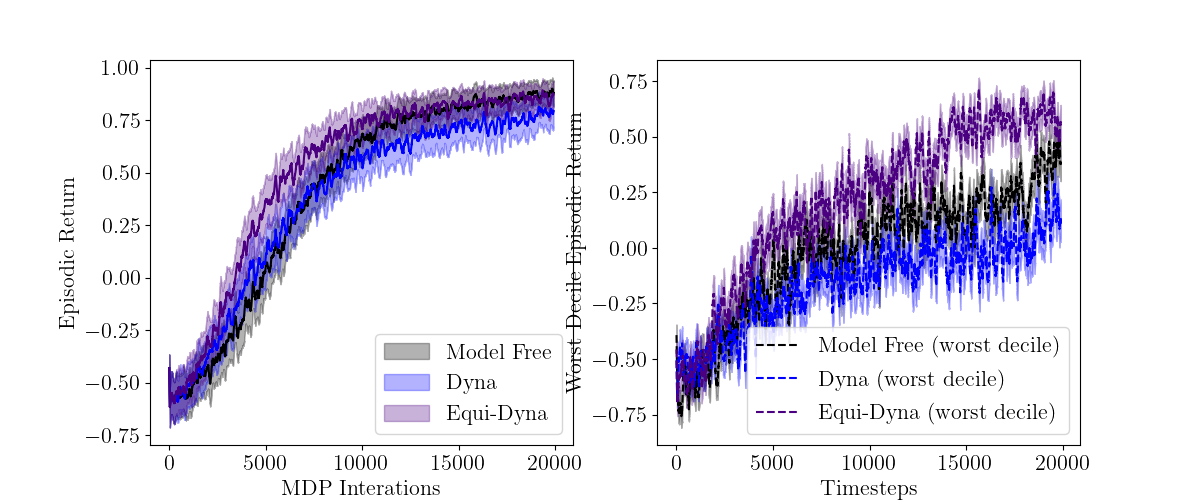
\includegraphics[width=\textwidth]{Figures/Expert_Dyna_Catch_pr4.png}
	\caption{Left: Mean episodic returns for the CartPole agents across 128 random seeds
		plotted against number of interaction time-steps in the MDP. Right: The mean
		cumulative episodic returns of the worst performing 128 random seeds against
		number of experience time-steps in the MDP. Both of the plots are moving
		averages, with windows of 10 time-steps. Additionally, two standard errors are
		plotted.}
	\label{fig:supervised-dyna-cp}
\end{figure}



\subsection{Catch}
In catch the transitions between states are much simpler with the updates to the ball position between timesteps.
\begin{equation}
	y_{t+1} = y_t + 1.
\end{equation}
And the paddle displacement is governed by,
\begin{equation}
	x_{t+1} = \text{clip}(1- a_t + x_t, 0, 5).
\end{equation}
Above the clip function, stops the paddle moving beyond the environment's boundaries. The observations from the environment are arrays of shape $5 , 10$, with two ones, indicating the ball and paddle position. The paddle is in row 9, and the ball is only allowed in rows $0 -8$. To encode these constraints the network parameterises two distributions over the ball and paddle locations. The ball can be in one of 45 states, and the paddle may be in one of 5 states. The outputs of the networks are then the logits of the two distributions. In order to predict the next state, the mode of the distributions is taken for both the ball and the paddle.

Again construction of the G-CNN is much the same as in the case for CartPole, the basic network built from group convolutions. Again two hidden layers are used. Typically for a network predicting distributions against logits, the Binary Cross Entropy loss is used, however, it was found that this was not as effective as using the L2 distance between the logits, and the observation. Thus the loss function to train both transition models was,
\begin{equation}
	L(\phi) = \frac{1}{N}\sum_{(s, a, s') \sim \tau}^N (1 - \delta(\text{done}))||T(s, a) - s'||_2 \end{equation} Here, the one subtlety is that the loss is only back propagated if $s$, is not a terminal state. The indicator function $\delta(\text{done}) = 1 \text{if $s$ is terminal} $. Thus the model only learns transitions goverend by the environment dynamics, and not how to reset the episode.

In order to make the model equivariant the proximal pooling layer a distance metric needs to be used that quantifies how far apart the predictions are. The metric used is an L1 loss between the x, y position in s and s' of both the ball and the paddle. Additionally, to make the possible number of distances greater when the distances are summed, the ball's displacement is multiplied by 0.13. This constant value was found to improve the equivariance behaviour of the proximal pooling layer. The distance metric is then given by,
\begin{equation}
	d(s, s') = ||\text{mode}(T(s, a)_b) - s'_b||_1 + 0.13 ||\text{mode}T(s, a)_p - s'_p||_1.
\end{equation}
The subscripts, $b, p$ indicate the ball and the paddle distributions respectively.

\subsubsection{Results: Comparing Convergence of Transition Models}
In the same manner as before for CartPole, the transition models were trained on three different datasets to asses their convergence behaviour. In the same vein these were a random and expert policy sampled data, only left actions from the previous dataset, and only random policy sampled transitions.
\begin{figure}\label{fig:transition_model_catch}
	\centering
	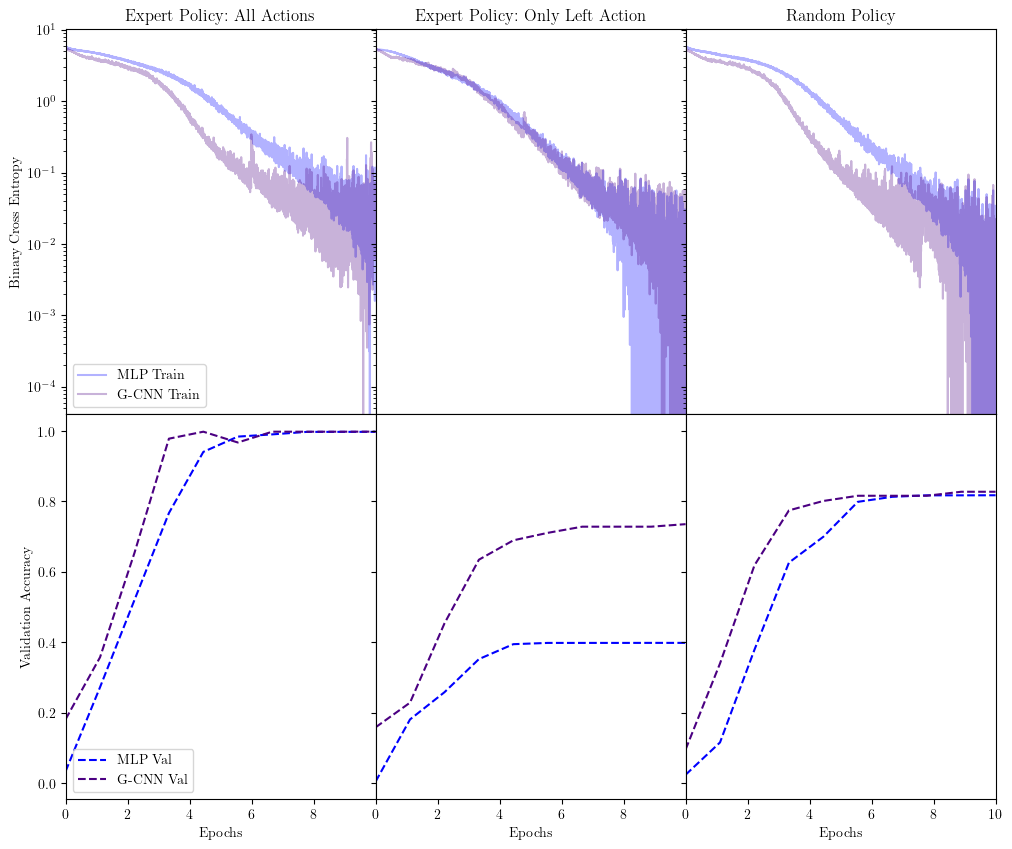
\includegraphics[width=\linewidth]{Figures/transition_model_catch.png}
	\label{fig:transition_model_catch}
	\caption{Transition Model BCE error, plotted against epochs for three different training datasets, With model validation accuracy plotted below. Left, the dataset contains a 50/50 split between expert policy sampled transitions, and transitions sampled from a random policy. Center, the same dataset as left, however, with only the left action taken. Right, solely transitions sampled from a random policy. These datasets contain 40,000 transitions. All plots have the same set of validation data with a 50/50 split of expert and radom policy sampled data.}
\end{figure}
In Fig.\ref{fig:transition_model_catch}, the equivariant model, again demonstrates the effectiveness of inductive biases. The Equivariant and MLP models achieve $0.998$ validation accuracy on transitions sampled from the joint expert random policy, with slightly faster convergence. When acting on a dataset, which has been filtered for only the left actions. The equivariant G-CNN generalizes to the right hand action much better than that of the MLP as expected. Clearly, the validation and training datasets are not disjoint, as the discrete state space is so small. Thus, it is not an accurate measure of performance on unseen states.

The random policy sampled dataset, doesn't include all possible states, that the environment begins in. In this case both models approach the fraction of the states present in the training as the validation set. As such, there appears to be little generalization to states not seen in the training data. Which in some way is not a problem, if the transition model can approach perfection, then the planning phase should be very effective.

\subsubsection{Results: Supervised-Dyna}
Again, three agents were trained over 128 random seeds, to compare the performance the equivariant G-CNN Dyna against an MLP and baseline actor-critic. The number of Dyna iterations was set to 25 for both the MLP transition model Dyna agent (Dyna), and the equivariant transition model (Equi-Dyna) agent. 25 was chosen, due to the results of the Ablation study found in~\ref{apd:supervised-dyna-cp}.

\begin{figure}
	\label{fig:supervised-dyna-catch}
	\centering
	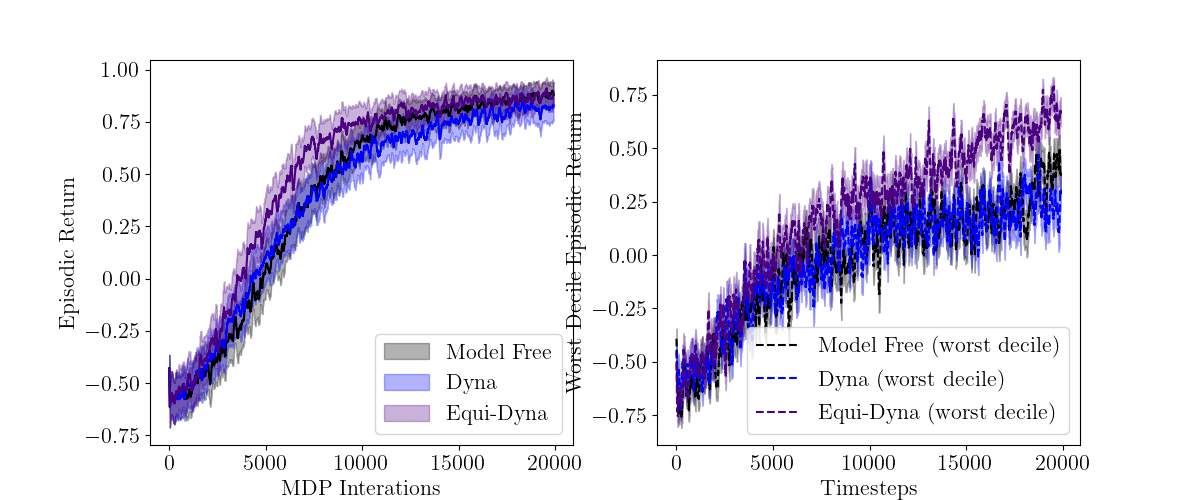
\includegraphics[width=\textwidth]{Figures/Expert_Dyna_Catch_pr2.png}
	\caption{Left: Mean episodic returns for the Catch agents across 128 random seeds
		plotted against number of interaction time-steps in the MDP. Right: The mean
		cumulative episodic returns of the worst performing 128 random seeds against
		number of experience time-steps in the MDP. Both of the plots are moving
		averages, with windows of 10 time-steps. Additionally, two standard errors are
		plotted.}
\end{figure}

Inspecting the returns in Fig.\ref{fig:supervised-dyna-catch} we see that the equivariant transition model dyna agent (Equi-Dyna), outperforms the baseline and the Dyna Model.

\subsection{Transition Model Conclusion}
For both Catch and CartPole the equivariant G-CNN transition models with a proximal pooling layer are able to match and or improve upon the MLP transition models. Further, there is sufficient evidence to believe that the proximal pooling layer suffices, with the correct distance metric, to produce approximately equivariant transition models. This can be seen in both Catch and CartPole, where there is a substantial uplift in accuracy or loss on unseen data. Due to the G-CNNs ability to generalize to states not seen in the training data, if these states are in the orbit of states in the training data.
